% !TeX root = ..

\subsection{
  Стратегии проектирования маршрута режущего инструмента
  для многоугольных заготовок
}
\label{sect:2.2.2}

В машиностроительном производстве
при раскрое листового материала с помощью машин лазерной резки с ЧПУ
к наиболее часто встречающимся геометрическим
типам заготовок,
помимо круглых внешних контуров,
относят также многоугольные заготовки --
часто выпуклые симметричные многоугольники с отверстиями различной формы.
К отдельной группе можно отнести треугольные и прямоугольные заготовки.
Следует отметить, что прямоугольные заготовки целесообразно обрабатывать
с помощью совмещенного реза.
Касательно остальных многоугольных (в т. ч. треугольных)
заготовок применение совмещенного реза неэффективно,
т. к. обычно с помощью одной точки врезки удается вырезать обычно две заготовки.
Также неэффективны другие специальные способы резки
(например, <<цепная>> резка или резка змейкой),
т. к. применение выделенных способов приводит к
сокращению количества точек врезок,
но
$L_{on}=\mathrm{const}$
что,
в свою очередь,
повышает время
$T_{cut}$
и стоимость раскроя
$F_{cost}$.
Поэтому возникает необходимость в разработке
новых специальных способов резки для выделенной группы заготовок.

В отдельную группу выделим треугольные заготовки,
для листовой резки которых на машине лазерной резки с ЧПУ
применим мультиконтурную резку,
соединяющую совмещенный рез и резку змейкой.
На рис.~\ref{6-6}
приведена схема резки шести треугольных заготовок
одного размера с помощью резки <<по замкнутому>> контуру, при этом
$N_{pt}=6$
(цифрами {\it 1--6}
обозначена последовательность резки).

\begin{figure}[H]
  \centering
  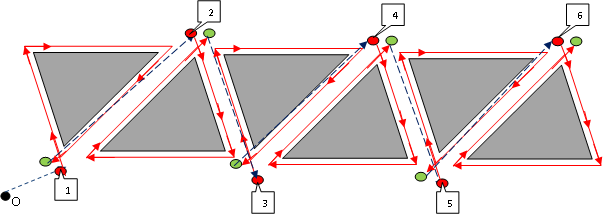
\includegraphics[width=0.9\textwidth]{6-6.png}
  \caption{
    Схема резки шести треугольных заготовок
    с помощью резки
    <<по~замкнутому контуру>>
  }
  \label{6-6}
\end{figure}

На рис.~\ref{6-1} приведена схема резки тех же шести
треугольных заготовок, при этом
$N_{pt}=1$.
Цифрами {\it 1--13} обозначена последовательность
резки контуров в одном сегменте,
т. е. после врезания в материал режущий инструмент
на рабочем ходу переходит к вырезке участка под номером {\it 1}
первого контура,
затем без дополнительного реза режущая головка
переходит ко второму контуру и вырезает участок под номером
{\it 2} и т. д.
В конце режущий инструмент завершает вырезку шести контуров
с одной точкой врезки по {\it 13} участку и переходит к
точке выключения инструмента.
Следует обратить внимание, что в рассматриваемом способе
резки инструмент переходит от одного контура к другому
на рабочем ходу с совмещенным резом,
за счет чего сокращается количество точек врезки $N_{pt}$,
расстояние перемещений инструмента на рабочем $L_{on}$
и холостом  $L_{off}$ ходах.

\begin{figure}[H]
  \centering
  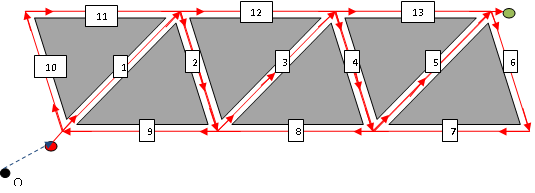
\includegraphics[width=0.9\textwidth]{6-1.png}
  \caption{
    Схема резки шести треугольных заготовок
    с помощью специального способа резки
  }
  \label{6-1}
\end{figure}

Способ резки, предложенный
на~рис.~\ref{6-1},
применим для групп треугольных заготовок одного типоразмера,
расположенных в два ряда.
При этом если количество рядов больше двух,
то создаются еще блоки заготовок,
каждый из которых включает в себя по два ряда треугольных заготовок.
Переход режущего инструмента от одного блока к другому
осуществляется с помощью холостого хода.
Внутри каждого блока реализована резка заготовок с одной точкой врезки.

В случае раскроя листового материала треугольными
заготовками можно спроектировать маршрут режущего
инструмента без холостого хода,
для этого треугольные заготовки необходимо
размещать согласно рис.~\ref{3-10}.
Основное условие непрерывной резки нескольких
заготовок заключается в том,
что общее количество пересекающихся ребер у
любой вершины треугольника должно быть четным.
Или, с точки зрения теории графов,
у каждой вершины
должно быть четное количество ребер.
В обратном случае непрерывную резку заготовок
с помощью одной точки врезки не осуществить
без дополнительных резов.
Например, как видно из рис.~\ref{3-10},
общее количество обозначенных цифрами
{\it 1, 2, 4, 5, 7} и {\it 8} ребер равно 6.

\begin{figure}[H]
  \centering
  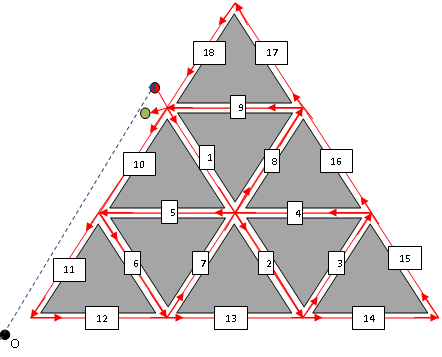
\includegraphics[width=0.8\textwidth]{3-10.png}
  \caption{
    Схема резки девяти треугольных заготовок
    с~помощью мультиконтурной~резки
  }
  \label{3-10}
\end{figure}

Цифрами {\it 1 -- 18} обозначена последовательность
резки контуров за один сегмент,
т. е. после врезания в материал режущий инструмент
на рабочем ходу переходит к вырезке участка
первого контура
(под номером {\it 1}),
затем без дополнительного реза режущая
головка переходит ко второму контуру и
вырезает участок под номером {\it 2} и т. д.
В конце режущий инструмент завершает
вырезку девяти контуров с одной точкой врезки
по {\it 18} участку и переходит к точке выключения инструмента.
Следует обратить внимание, что в рассматриваемом способе
резки инструмент переходит от одного контура к
другому на рабочем ходу с совмещенным резом,
за счет чего сокращается количество точек врезки $N_{pt}$,
расстояние перемещений инструмента на рабочем ходу  $L_{on}$,
при этом
$L_{off} \approx 0$.
Холостой переход осуществляется
только при переходе режущего инструмента
от нулевой точки до точки врезки и от
точки выключения инструмента до нулевой точки.
Способом, приведенным на рис. \ref{3-10},
можно размещать большое количество
треугольных заготовок, при этом всегда $N_{pt}=1$
и $L_{off} \approx 0$.

Предложенные выше методы резки применимы для любых треугольников.

Обработку пятиугольных заготовок из листового материала
на машине лазерной резки с ЧПУ также можно осуществить
предложенным методом, приведенным
на~рис.~\ref{6-1}
с помощью мультиконтурной резки,
объединяющей совмещенный рез и резку змейкой.
На рис.~\ref{5-6}
приведена схема резки <<по~замкнутому>> контуру
шести пятиугольных заготовок,
при этом $N_{pt}=6$.

\begin{figure}[H]
  \centering
  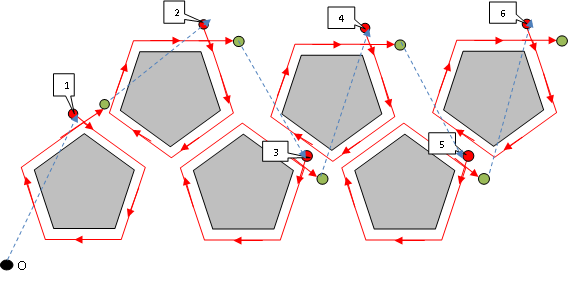
\includegraphics[width=0.9\textwidth]{5-6.png}
  \caption{
    Схема резки <<по замкнутому контуру>>
    шести пятиугольных заготовок
  }
  \label{5-6}
\end{figure}

На рис.~\ref{5-1}
предложена схема резки тех же шести
пятиугольных заготовок за один сегмент, при этом
$N_{pt}=1$
и $L_{off} \approx 0$.
С ее помощью
можно осуществлять резку по ребрам многоугольников,
соблюдая последовательность и направление резки каждого ребра.
Ход реза обозначен цифрами {\it 1--25}.
Инструмент перемещается на холостом ходу от
начальной точки положения инструмента
(точки {\it О})
до точки врезки, после чего осуществляется непрерывная резка всех ребер,
начиная с {\it 1},
без дополнительных резов за один сегмент.
После того как режущий инструмент частично вырежет
первый контур по четырем ребрам (с {\it 1} по {\it 4}),
он переходит к ребру {\it 5} и начинает вырезать
второй контур, последовательно вырезая с {\it 6} по {\it 9} ребра.
При вырезке {\it 9} ребра будут окончательно
вырезаны первый и второй контуры.
Аналогично можно вырезать оставшиеся контуры,
после чего инструмент переходит в точку выключения инструмента.

Как видно из рис.~\ref{5-1},
за счет применения совмещенного реза сокращается $L_{on}$,
за счет отсутствия холостых переходов
$L_{off} \approx 0$
и $N_{pt}=1$
при одновременном сокращении общего времени
и стоимости резки заготовок из листового
материала на машинах лазерной резки с ЧПУ.
Предложенный способ резки применим для любых выпуклых пятиугольников.

\begin{figure}[H]
  \centering
  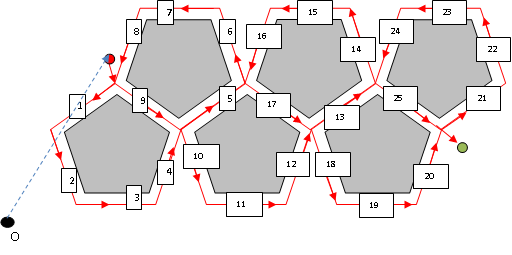
\includegraphics[width=0.9\textwidth]{5-1.png}
  \caption{
    Схема резки шести пятиугольных заготовок
    с применением мультиконтурной резки
  }
  \label{5-1}
\end{figure}

В случае обработки четырехугольных заготовок
целесообразно применять совмещенный рез
либо технологию, предложенную
на~рис.~\ref{5-1},
при условии, что общее количество ребер,
пересекающихся в любой внутренней вершине, будет четным.
В последнем случае значения
$N_{pt}$
и $L_{off}$
при использовании разработанного способа резки будут,
как правило, ниже, чем при совмещенном резе.
Но данный способ резки не всегда применим
с точки зрения снижения КИМ.

В общем случае при резке любых многоугольных
заготовок для случая,
когда количество пересекающихся ребер у вершин
(в частности внутренних) нечетно,
то предложенный способ резки реализуем с
дополнительным резом, либо с добавлением точек врезки.
Следует обратить внимание на то,
что при мультиконтурной резке многоугольников с
дополнительным резом значение
$L_\text{доп}^\text{факт}$
также как и для треугольников должно удовлетворять условию
$L_\text{доп}^\text{факт} \leqslant L_\text{доп}$,
рассчитанному по (\ref{l-fact-dop}),
а иначе значения целевых функций (\ref{cutting-time})
и (\ref{cutting-cost})
окажутся больше значений,
получаемых  при резке <<по замкнутому контуру>>.
На рис.~\ref{5-extra}
для любой вершины количество пересекающихся ребер нечетно,
поэтому резка контуров возможна только с дополнительным резом.

\begin{figure}[H]
  \centering
  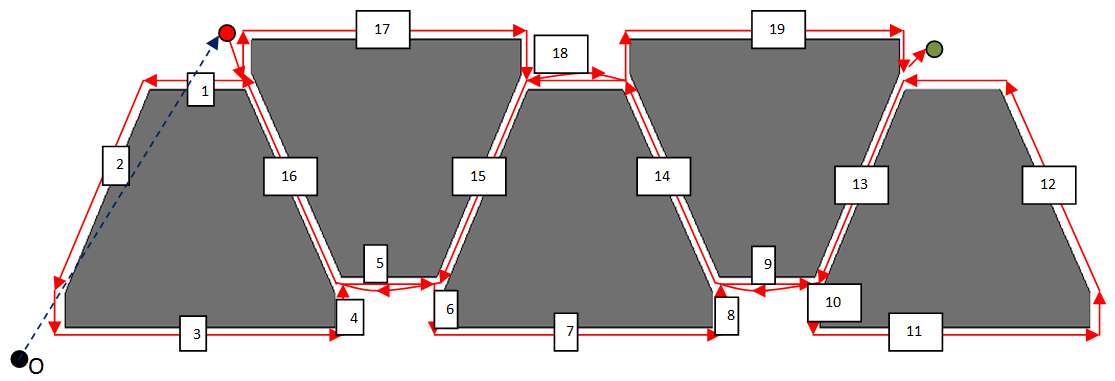
\includegraphics[width=0.9\textwidth]{5-extra.png}
  \caption{
    Схема резки пяти заготовок
    с помощью мультиконтурной резки
    с~дополнительным резом
    }
  \label{5-extra}
\end{figure}

Цифрами {\it 1--19} обозначена последовательность обхода ребер
пяти заготовок.
Режущий инструмент на холостом ходу переходит
из начальной точки в точку врезки,
после чего по эквидистантому контуру
осуществляется частичная вырезка первого
контура по ребрам {\it 1--4},
затем вырезается ребро {\it 5} второй заготовки и т. д.,
пока окончательно не будут вырезаны пять заготовок по ребрам
{\it 6--19}.
По причине наличия дополнительных резов рабочая
длина перемещения режущего инструмента может увеличиться по сравнению с $L_{on}$,
полученной в результате применения резки <<по замкнутому контуру>>,
поэтому актуален вопрос проверки неравенства
$L_\text{доп}^\text{факт} \leqslant L_\text{доп}$.
В результате применения предложенного на рис.~\ref{5-extra}
специального метода резки
$N_{pt}=1$
и $L_{off} \approx 0$.

Рассмотрим пример раскроя листового материала
{\it 12Х18Н10Т}
($\Delta$ = 1--8 мм)
многоугольными заготовками на машине лазерной резки с ЧПУ.
Для этого разработаны две раскройные карты с одинаковым количеством,
видом и размерами деталей,
для которых спроектирован маршрут перемещения
режущего инструмента в САПР <<Сириус>> с
применением резки <<по замкнутому контуру>>
(рис.~\ref{multi-a})
и специальной техники резки для многоугольных заготовок
(рис.~\ref{multi-b}).
Маршрут резки в обоих случаях
начинается в левом нижнем углу листа.

Полученные результаты, которые содержат значения
$L_{on}$, $N_{pt}$, $L_{off}$, $T_{cut}$ и $F_{cost}$
для каждой раскройной карты, приведены
в~табл.~\ref{polygons}
на стр.~\pageref{polygons}.

\begin{figure}[H]
  \centering
  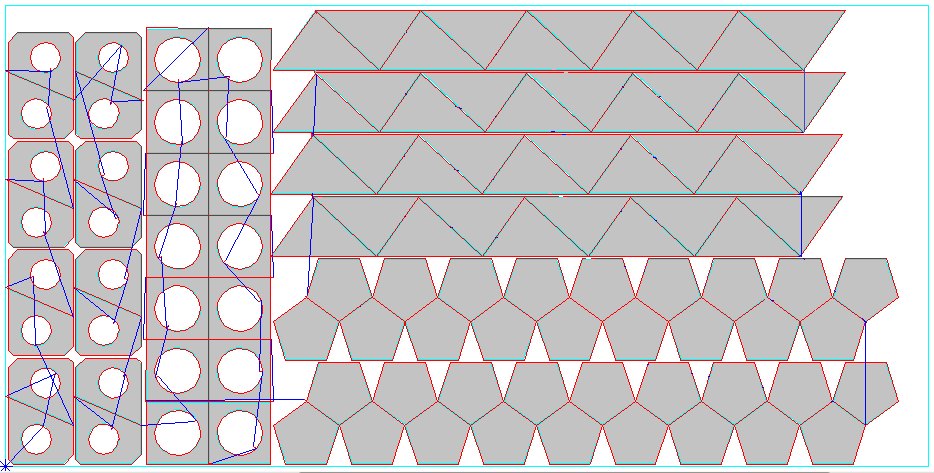
\includegraphics[width=0.9\textwidth]{multi-a.png}
  \caption{
    Схема раскройной карты
    с применением мультиконтурной резки
    для~многоугольных заготовок
  }
  \label{multi-a}
\end{figure}

\begin{figure}[H]
  \centering
  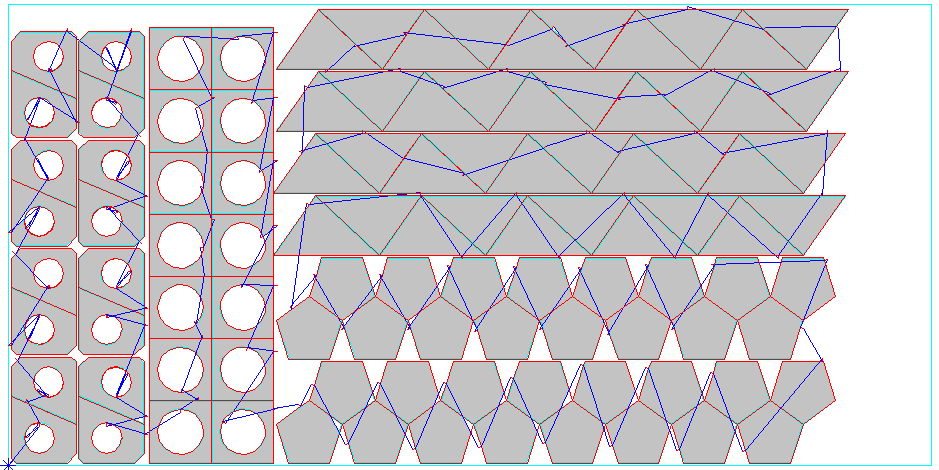
\includegraphics[width=0.9\textwidth]{multi-b.png}
  \caption{Схема раскройной карты с применением резки <<по замкнутому контуру>>}
  \label{multi-b}
\end{figure}

Применение предложенных специальных методов резки
приводит к значительному сокращению значений
$N_{pt}$, $L_{on}$ и $L_{off}$
в сравнении со стандартной техникой резки
соответственно до 70 \%, 27 \% и 67 \%
при одновременном сокращении времени
$T_{cut}$
и стоимости лазерной резки
$F_{cost}$ до 36 \%.
Как показывает практика применения
предложенных методов резки при проектировании
УП в реальном производственном процессе,
в среднем значения параметров
$L_{on}$, $N_{pt}$  и $L_{off}$
сокращаются на 3 \%, 60 \% и 65 \%
соответственно при одновременном снижении
$F_{cost}$
на 10--20 \%
по сравнению с резкой <<по замкнутому контуру>>.
Как видно из табл.~\ref{polygons}
с увеличением толщины обрабатываемого материала
сокращается эффективность предложенных специальных способов резки.

\begin{table}[H]
  \caption{
    Результаты расчета стоимости резки раскройного плана
    для~многоугольных заготовок
    }
  \label{polygons}
  \centering
  \begin{tabular}{c *{7}{|c}}
    \hline
    Марка & $\Delta$ & Резка &
      \shortstack{$L_{on}$, \\ м} &
      \shortstack{$L_{off}$, \\ м} &
      $N_{pt}$ &
      \shortstack{$F_{cost}$, \\ руб} &
      \% \\
    \hline
    \multirow{2}{*}{12Х18Н10Т} & \multirow{2}{*}{1 мм} & Стандартная & 101,85 & 26,92 & 163 & 2956,14 & \multirow{2}{*}{36,0} \\
    & & Специальная & 74,73 & 8,90 & 51 & 1901,4 \\
    \multirow{2}{*}{12Х18Н10Т} & \multirow{2}{*}{3 мм} & Стандартная & 101,85 &	26,92 & 163 & 9170,09 & \multirow{2}{*}{36,5} \\
    & & Специальная & 74,73 & 8,90 & 51 & 5823,10 \\
    \multirow{2}{*}{12Х18Н10Т} & \multirow{2}{*}{5 мм} & Стандартная & 101,85 & 26,92 & 163 & 23262,44 & \multirow{2}{*}{32,2} \\
    & & Специальная & 74,73 & 8,90 & 51 & 15768,17 \\
    \multirow{2}{*}{12Х18Н10Т} & \multirow{2}{*}{8 мм} & Стандартная & 101,85 & 26,92 & 163 & 94070,86 & \multirow{2}{*}{29,7} \\
    & & Специальная & 74,73 & 8,90 & 51 & 66121,93 \\
    \hline
  \end{tabular}
\end{table}

Таким образом, можно сделать следующие выводы.

\begin{enumerate}
\item
Применение специальных методов резки
для различных многоугольных заготовок возможно
без дополнительных резов между заготовками при условии,
что количество пересекающихся ребер у вершин
(в частности, внутренних) четно.
В остальных случаях резка разработанным
способом возможна с дополнительным резом,
либо с увеличением числа точек врезки.
Предложенные методы базируются на известных методах резки
(змейкой и совмещенный рез),
за счет этого значительно сокращаются
значения основных параметры
$L_{on}$, $N_{pt}$  и $L_{off}$
при одновременном снижении
$T_{cut}$
и
$F_{cost}$.

\item
В зависимости от типа заготовок,
наличия или отсутствия отверстий в деталях
количество точек врезки может снизиться до
$N_{pt}=1$,
при этом
$L_{off} \approx 0$.
В рассмотренных примерах значения
$N_{pt}$, $L_{off}$ и $L_{on}$
максимально сокращаются соответственно до 70 \%, 67 \% и 27 \%
при одновременном сокращении
$T_{cut}$
и
$F_{cost}$
до 36 \%.
В среднем значение $F_{cost}$ снижается на 10--20 \%.

\item
При применении предложенных специальных способов резки
для многоугольных деталей с дополнительным резом
необходимо вычислить значение
$L_\text{доп}^\text{факт}$:
$L_\text{доп}^\text{факт} \leqslant L_\text{доп}$.
В противном случае значение
$L_\text{доп}$
может оказаться больше значения
$L_{on}$,
полученное при резке <<по замкнутому контуру>>,
что,
в свою очередь,
может привести к увеличению значений целевых функций
$T_{cut}$
и
$F_{cost}$.

\item Эффективность применения предложенных способов резки
сокращается при увеличении толщины обрабатываемого материала.
\end{enumerate}

Отметим, что
предложенные способы применения специальных техник резки и
формирование групп однотипных заготовок на этапе
проектирования раскроя листовых материалов на фигурные заготовки,
среди которых присутствуют круглые и многоугольные,
можно интерпретировать как методы формирования наборов базовых сегментов
(а в дискретном случае – мегаполисов)
для последующего решения задач оптимизации класса
{\it GSCCP}
средней и большой размерности.
Это создает,
в свою очередь,
предпосылки  для разработки эффективных методов
решения интегрированной задачи раскроя и маршрутизации,
для которой целевая функция стоимости складывается
из стоимости использованного материала для раскроя
и стоимости процесса резки
$
F_{cost}=
L_{on} \cdot C_{on} +
L_{off} \cdot C_{off} +
N_{pt} \cdot C_{pt}
$.
